\section{Последовательность работы торгового представителя с планшетным\\ устройством}
\begin{enumerate}[\thesection .1]
\item Рабочий день торгового представителя в части работы с планшетным ПК \footnote{В рамках данного документа под термином планшетный ПК подразумевается карманный персональный компьютер на базе ОС Android.}, начинается с проверки уровня заряда. В случае если уровень заряда планшетного ПК недостаточен для обеспечения бесперебойной работы до обеденного перерыва (это может определяться индивидуально для каждого планшета, но можно ориентироваться на уровень заряда более 90\% ) необходимо обеспечить процесс зарядки планшета путём подключения его к сети переменного тока, либо к зарядному устройству автомобиля.

\begin{figure}[h]
	\begin{floatrow}
		\ffigbox{\caption{Значок заряда}\label{pic:pic1}}%
		{
\includegraphics[width=0.5\linewidth]{scr1.jpg}}
		\ffigbox{\caption{Значок GPS}\label{pic:pic2}}%
		{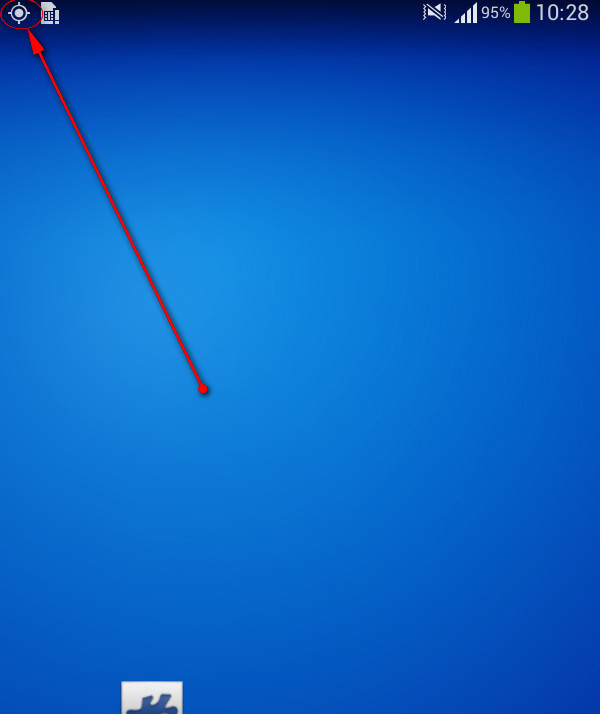
\includegraphics[width=0.5\linewidth]{scr2.jpg}}         
	\end{floatrow}
\end{figure}

Уровень заряда планшета в общем случае можно определить по значку «батарейки» расположенному в правом верхнем углу экрана.(рис.\ref{pic:pic1})
%\hyperref[pic:pic1]{рис.}
\item Затем торговый представитель должен определить включён ли у планшета модуль GPS.
При включённом модуле GPS  на самой верхней строчке экрана планшета, отображается значок GPS
(рис.\ref{pic:pic2})
\item После этого необходимо запустить программу «Оптимум» иконка которой расположена на рабочем столе планшета торгового представителя.Запуск программы осуществляется путём «тапа»(прикосновения к иконке программы).
(рис.\ref{pic:pic3})
\begin{figure}[h]
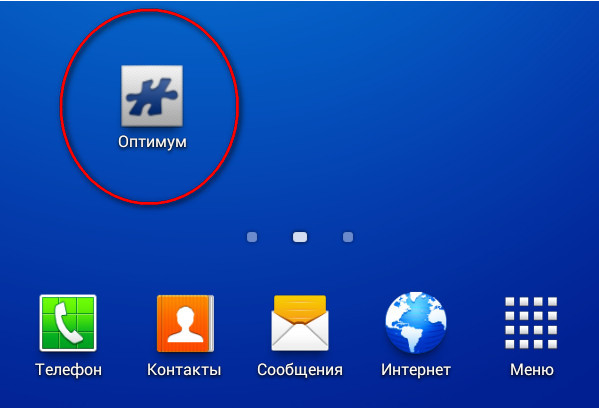
\includegraphics[width=0.3\linewidth]{scr3.jpg} 
\caption{<<Иконка>> Оптимы}\label{pic:pic3}
\end{figure}

\item При запуске программы пользователь попадает в главное меню <<Оптимы>>\label{it:it2_1}
(рис.\ref{pic:picgl})
\begin{figure}[h]
	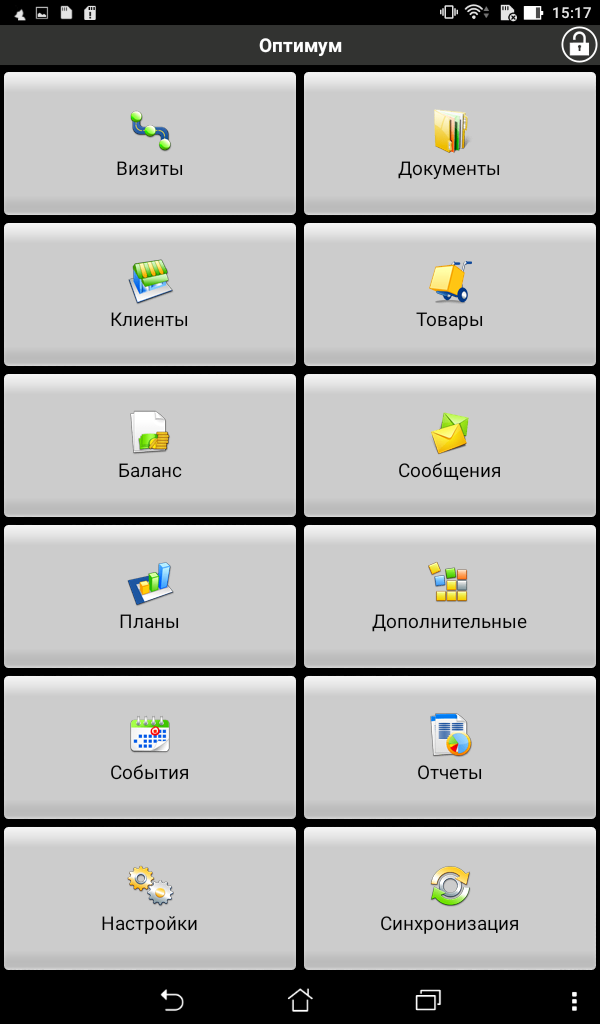
\includegraphics[width=0.2\linewidth]{scr_gl.png} 
	\caption{Главное меню <<Оптимы>>}\label{pic:picgl}
\end{figure}


\item Далее торговый представитель нажимает кнопку «Синхронизация»(рис.\ref{pic:pic4})
и попадает в раздел «Синхронизация».
(рис.\ref{pic:pic5})
\begin{figure}[h]
  \begin{floatrow}
   \ffigbox{\caption{Меню синхронизация}\label{pic:pic4}}%
           {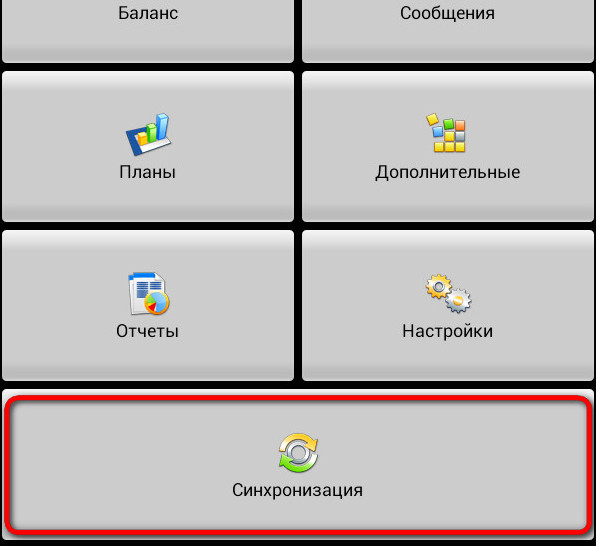
\includegraphics[width=0.8\linewidth]{scr4.jpg}}
   \ffigbox{\caption{Раздел синхронизация}\label{pic:pic5}}%
           {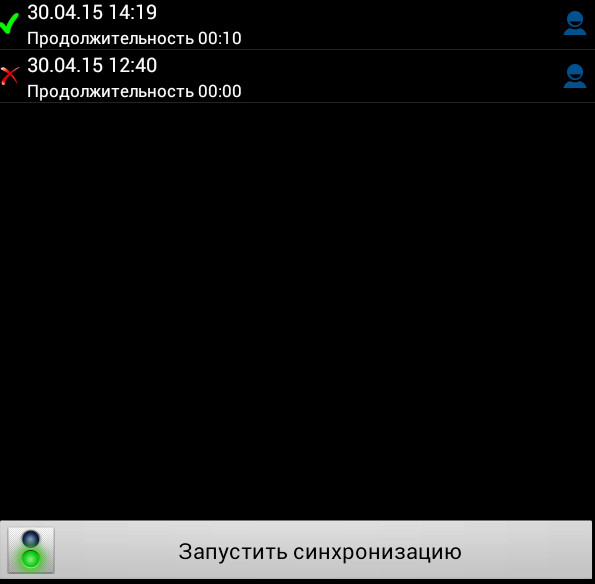
\includegraphics[width=0.75\linewidth]{scr5.jpg}}         
  \end{floatrow}
\end{figure}
%http://mydebianblog.blogspot.ru/2013/06/floatrow-figures-in-a-row.html
%http://mydebianblog.blogspot.ru/2013/06/floatrow-caption-position.html
\item В этом разделе торговый представитель, используя кнопку «Запустить синхронизацию» \label{it:it2_2}
(рис.\ref{pic:pic6})
совершает запуск синхронизации и дожидается ее окончания.(рис.\ref{pic:pic7}) 
\begin{figure}[!h]
	\begin{floatrow}
		\ffigbox{\caption{Запуск синхронизации}\label{pic:pic6}}%
		{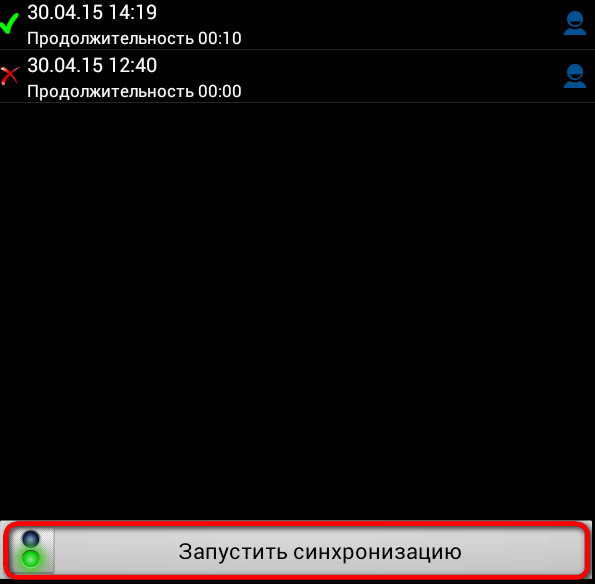
\includegraphics[width=0.8\linewidth]{scr6.jpg}}
		\ffigbox{\caption{Процесс синхронизации}\label{pic:pic7}}%
		{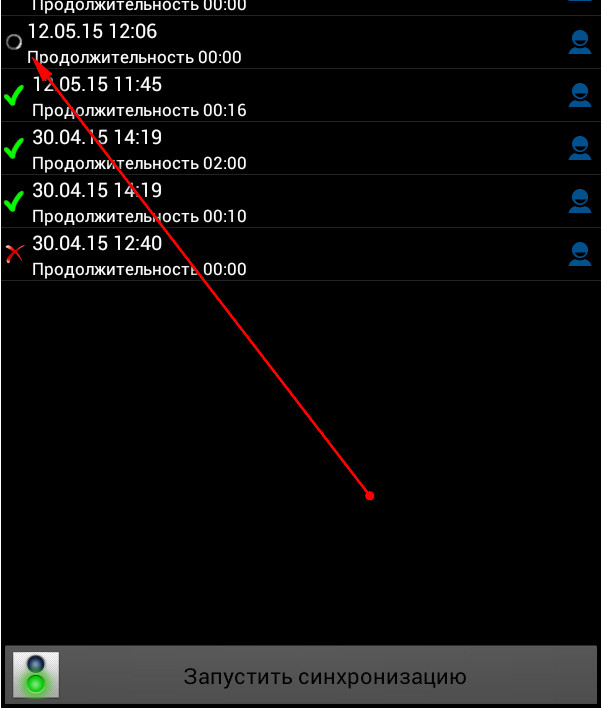
\includegraphics[width=0.75\linewidth]{scr7.jpg}}         
	\end{floatrow}
\end{figure}

Об успешном прохождении синхронизации свидетельствует «зелёная галочка» слева от строки с выполнявшейся синхронизацией.(рис.\ref{pic:pic8}) 
\begin{figure}[!h]
	\begin{floatrow}
		\ffigbox{\caption{Синхронизация успешна}\label{pic:pic8}}%
		{
\includegraphics[width=0.8\linewidth]{scr8.jpg}}
		\ffigbox{\caption{Синхронизация неудачна}\label{pic:pic9}}%
		{
\includegraphics[width=0.75\linewidth]{scr9.jpg}}         
	\end{floatrow}
\end{figure}
\item Если отображается значок «красный крестик» (рис.\ref{pic:pic9}) это означает, что синхронизация «не прошла». 
В таком случае необходимо удостовериться, что на планшетном ПК включена  передача «мобильные данные» и повторить синхронизацию согласно  п. \ref{it:it2_2}
\item Если несколько раз подряд выполнение синхронизации не было успешным, необходимо «перезагрузить» планшет. Т.е. выключить его и повторно включить спустя 2-3 минуты. Затем повторить пункты с \ref{it:it2_1} по \ref{it:it2_2}
\item После этих действий планшетный ПК готов к работе.
\end{enumerate}